\documentclass[a4paper, 12pt]{article}
\usepackage[T2A]{ fontenc }
\usepackage[utf8]{ inputenc }
\usepackage[english, russian]{babel}
\usepackage{amsmath,amsfonts,amssymb,amsthm,mathtools}
\usepackage[colorlinks, linkcolor = blue]{hyperref}
\usepackage{upgreek}
\usepackage[left = 2cm, right = 2cm, top = 2cm, bottom = 3cm, bindingoffset = 0cm]{geometry}
\usepackage{graphicx}
\usepackage{multirow}
\usepackage{xcolor}
\usepackage{tabularx}
\title{ Differenciator }
\author{Valiev Ruzal}
\date{December 2023}
\begin{document}
\maketitle
\section{Expression}
By applying the chain rule...\newline
$ sin( x )  +  cos(  { x } ^ {\small 2 }  ) $\newline
By employing combinatorial arguments...\newline
$ sin( x )  +  cos(  { x } ^ {\small 2 }  ) $\newline
Considering the behavior of the function at critical points.\newline
$ sin( x )  +  cos(  { x } ^ {\small 2 }  ) $\newline
Let's examine the case when the variables are independent.\newline
$ cos( x )  + -1 \cdot  sin(  { x } ^ {\small 2 }  )  \cdot 2 \cdot x$\newline
We'll determine the domain and range of the function.\newline
$ cos( x )  + -1 \cdot  sin(  { x } ^ {\small 2 }  )  \cdot 2 \cdot x$\newline
Considering the behavior of the function at critical points.\newline
$-1 \cdot  sin( x )  \cdot 1 + 0 +  ( 0 + -1 \cdot  cos(  { x } ^ {\small 2 }  )  \cdot 2 \cdot x )  \cdot 2 \cdot x + -1 \cdot  sin(  { x } ^ {\small 2 }  )  \cdot  ( 0 + 2 \cdot 0 \cdot  { x } ^ {\small  ( 1 - 1 )  }  + 0 ) $\newline
Let's investigate the convergence/divergence of this series.\newline
$-1 \cdot  sin( x )  \cdot 1 + -1 \cdot  cos(  { x } ^ {\small 2 }  )  \cdot 2 \cdot x \cdot 2 \cdot x + -1 \cdot  sin(  { x } ^ {\small 2 }  )  \cdot  ( 0 + 2 \cdot 0 ) $\newline
Let's investigate the convergence/divergence of this series.\newline
$-1 \cdot  sin( x )  + -1 \cdot  cos(  { x } ^ {\small 2 }  )  \cdot 2 \cdot x \cdot 2 \cdot x + -1 \cdot  sin(  { x } ^ {\small 2 }  )  \cdot 0$\newline
We'll simplify the expression by factoring.\newline
$-1 \cdot  sin( x )  + -1 \cdot  cos(  { x } ^ {\small 2 }  )  \cdot 2 \cdot x \cdot 2 \cdot x + 0$\newline
Considering the behavior of the function at critical points.\newline
$-1 \cdot  sin( x )  + -1 \cdot  cos(  { x } ^ {\small 2 }  )  \cdot 2 \cdot x \cdot 2 \cdot x$\newline
We'll establish a correspondence between...\newline
$-1 \cdot  sin( x )  + -1 \cdot  cos(  { x } ^ {\small 2 }  )  \cdot 2 \cdot x \cdot 2 \cdot x$\newline
We'll establish a correspondence between...\newline
$0 + -1 \cdot  cos( x )  + 0 + 0 + 0 + 0 +  ( 0 + 0 + 0 + -1 \cdot  ( -1 \cdot  sin(  { x } ^ {\small 2 }  )  \cdot 2 \cdot x \cdot 2 \cdot x +  cos(  { x } ^ {\small 2 }  )  \cdot  ( 0 + 2 \cdot 0 \cdot  { x } ^ {\small  ( 1 - 1 )  }  + 0 )  )  )  \cdot 2 \cdot x +  ( 0 + -1 \cdot  cos(  { x } ^ {\small 2 }  )  \cdot 2 \cdot x )  \cdot  ( 0 + 2 \cdot 0 \cdot  { x } ^ {\small  ( 1 - 1 )  }  + 0 )  +  ( 0 + -1 \cdot  cos(  { x } ^ {\small 2 }  )  \cdot 2 \cdot x )  \cdot  ( 0 + 2 \cdot 0 \cdot  { x } ^ {\small  ( 1 - 1 )  }  + 0 )  + -1 \cdot  sin(  { x } ^ {\small 2 }  )  \cdot  ( 0 + 0 + 0 + 2 \cdot  ( 0 + 0 + 0 )  + 0 + 0 + 0 ) $\newline
By applying the chain rule...\newline
$0 + -1 \cdot  cos( x )  + 0 +  ( 0 + -1 \cdot  ( -1 \cdot  sin(  { x } ^ {\small 2 }  )  \cdot 2 \cdot x \cdot 2 \cdot x +  cos(  { x } ^ {\small 2 }  )  \cdot  ( 0 + 2 \cdot 0 )  )  )  \cdot 2 \cdot x + -1 \cdot  cos(  { x } ^ {\small 2 }  )  \cdot 2 \cdot x \cdot  ( 0 + 2 \cdot 0 )  + -1 \cdot  cos(  { x } ^ {\small 2 }  )  \cdot 2 \cdot x \cdot  ( 0 + 2 \cdot 0 )  + -1 \cdot  sin(  { x } ^ {\small 2 }  )  \cdot  ( 0 + 2 \cdot 0 + 0 ) $\newline
By employing combinatorial arguments...\newline
$0 + -1 \cdot  cos( x )  + -1 \cdot  ( -1 \cdot  sin(  { x } ^ {\small 2 }  )  \cdot 2 \cdot x \cdot 2 \cdot x +  cos(  { x } ^ {\small 2 }  )  \cdot 0 )  \cdot 2 \cdot x + -1 \cdot  cos(  { x } ^ {\small 2 }  )  \cdot 2 \cdot x \cdot 0 + -1 \cdot  cos(  { x } ^ {\small 2 }  )  \cdot 2 \cdot x \cdot 0 + -1 \cdot  sin(  { x } ^ {\small 2 }  )  \cdot  ( 0 + 0 ) $\newline
By applying the chain rule...\newline
$-1 \cdot  cos( x )  + -1 \cdot  ( -1 \cdot  sin(  { x } ^ {\small 2 }  )  \cdot 2 \cdot x \cdot 2 \cdot x + 0 )  \cdot 2 \cdot x + 0 + 0 + 0$\newline
By applying the chain rule...\newline
$-1 \cdot  cos( x )  + -1 \cdot -1 \cdot  sin(  { x } ^ {\small 2 }  )  \cdot 2 \cdot x \cdot 2 \cdot x \cdot 2 \cdot x + 0$\newline
We'll establish a correspondence between...\newline
$-1 \cdot  cos( x )  + -1 \cdot -1 \cdot  sin(  { x } ^ {\small 2 }  )  \cdot 2 \cdot x \cdot 2 \cdot x \cdot 2 \cdot x$\newline
We'll simplify the expression by factoring.\newline
$-1 \cdot  cos( x )  + -1 \cdot -1 \cdot  sin(  { x } ^ {\small 2 }  )  \cdot 2 \cdot x \cdot 2 \cdot x \cdot 2 \cdot x$\newline
By employing combinatorial arguments...\newline
$0 + 0 + 0 + -1 \cdot  ( -1 \cdot  sin( x )  \cdot 1 + 0 )  + 0 + 0 + 0 + 0 + 0 + 0 + 0 + 0 + 0 + 0 +  ( 0 + 0 + 0 + 0 + 0 + 0 + 0 + -1 \cdot  (  (  ( 0 + -1 \cdot  cos(  { x } ^ {\small 2 }  )  \cdot 2 \cdot x )  \cdot 2 \cdot x + -1 \cdot  sin(  { x } ^ {\small 2 }  )  \cdot  ( 0 + 2 \cdot 0 \cdot  { x } ^ {\small  ( 1 - 1 )  }  + 0 )  )  \cdot 2 \cdot x + -1 \cdot  sin(  { x } ^ {\small 2 }  )  \cdot 2 \cdot x \cdot  ( 0 + 2 \cdot 0 \cdot  { x } ^ {\small  ( 1 - 1 )  }  + 0 )  + -1 \cdot  sin(  { x } ^ {\small 2 }  )  \cdot 2 \cdot x \cdot  ( 0 + 2 \cdot 0 \cdot  { x } ^ {\small  ( 1 - 1 )  }  + 0 )  +  cos(  { x } ^ {\small 2 }  )  \cdot  ( 0 + 0 + 0 + 2 \cdot  ( 0 + 0 + 0 )  + 0 + 0 + 0 )  )  )  \cdot 2 \cdot x +  ( 0 + 0 + 0 + -1 \cdot  ( -1 \cdot  sin(  { x } ^ {\small 2 }  )  \cdot 2 \cdot x \cdot 2 \cdot x +  cos(  { x } ^ {\small 2 }  )  \cdot  ( 0 + 2 \cdot 0 \cdot  { x } ^ {\small  ( 1 - 1 )  }  + 0 )  )  )  \cdot  ( 0 + 2 \cdot 0 \cdot  { x } ^ {\small  ( 1 - 1 )  }  + 0 )  +  ( 0 + 0 + 0 + -1 \cdot  ( -1 \cdot  sin(  { x } ^ {\small 2 }  )  \cdot 2 \cdot x \cdot 2 \cdot x +  cos(  { x } ^ {\small 2 }  )  \cdot  ( 0 + 2 \cdot 0 \cdot  { x } ^ {\small  ( 1 - 1 )  }  + 0 )  )  )  \cdot  ( 0 + 2 \cdot 0 \cdot  { x } ^ {\small  ( 1 - 1 )  }  + 0 )  +  ( 0 + -1 \cdot  cos(  { x } ^ {\small 2 }  )  \cdot 2 \cdot x )  \cdot  ( 0 + 0 + 0 + 2 \cdot  ( 0 + 0 + 0 )  + 0 + 0 + 0 )  +  ( 0 + 0 + 0 + -1 \cdot  ( -1 \cdot  sin(  { x } ^ {\small 2 }  )  \cdot 2 \cdot x \cdot 2 \cdot x +  cos(  { x } ^ {\small 2 }  )  \cdot  ( 0 + 2 \cdot 0 \cdot  { x } ^ {\small  ( 1 - 1 )  }  + 0 )  )  )  \cdot  ( 0 + 2 \cdot 0 \cdot  { x } ^ {\small  ( 1 - 1 )  }  + 0 )  +  ( 0 + -1 \cdot  cos(  { x } ^ {\small 2 }  )  \cdot 2 \cdot x )  \cdot  ( 0 + 0 + 0 + 2 \cdot  ( 0 + 0 + 0 )  + 0 + 0 + 0 )  +  ( 0 + -1 \cdot  cos(  { x } ^ {\small 2 }  )  \cdot 2 \cdot x )  \cdot  ( 0 + 0 + 0 + 2 \cdot  ( 0 + 0 + 0 )  + 0 + 0 + 0 )  + -1 \cdot  sin(  { x } ^ {\small 2 }  )  \cdot  ( 0 + 0 + 0 + 0 + 0 + 0 + 0 + 2 \cdot  ( 0 + 0 + 0 + 0 + 0 + 0 + 0 )  + 0 + 0 + 0 + 0 + 0 + 0 + 0 ) $\newline
It's essential to consider the implications of this axiom.\newline
$0 + -1 \cdot -1 \cdot  sin( x )  \cdot 1 + 0 + 0 + 0 +  ( 0 + 0 + -1 \cdot  (  ( -1 \cdot  cos(  { x } ^ {\small 2 }  )  \cdot 2 \cdot x \cdot 2 \cdot x + -1 \cdot  sin(  { x } ^ {\small 2 }  )  \cdot  ( 0 + 2 \cdot 0 )  )  \cdot 2 \cdot x + -1 \cdot  sin(  { x } ^ {\small 2 }  )  \cdot 2 \cdot x \cdot  ( 0 + 2 \cdot 0 )  + -1 \cdot  sin(  { x } ^ {\small 2 }  )  \cdot 2 \cdot x \cdot  ( 0 + 2 \cdot 0 )  +  cos(  { x } ^ {\small 2 }  )  \cdot  ( 0 + 2 \cdot 0 + 0 )  )  )  \cdot 2 \cdot x +  ( 0 + -1 \cdot  ( -1 \cdot  sin(  { x } ^ {\small 2 }  )  \cdot 2 \cdot x \cdot 2 \cdot x +  cos(  { x } ^ {\small 2 }  )  \cdot  ( 0 + 2 \cdot 0 )  )  )  \cdot  ( 0 + 2 \cdot 0 )  +  ( 0 + -1 \cdot  ( -1 \cdot  sin(  { x } ^ {\small 2 }  )  \cdot 2 \cdot x \cdot 2 \cdot x +  cos(  { x } ^ {\small 2 }  )  \cdot  ( 0 + 2 \cdot 0 )  )  )  \cdot  ( 0 + 2 \cdot 0 )  + -1 \cdot  cos(  { x } ^ {\small 2 }  )  \cdot 2 \cdot x \cdot  ( 0 + 2 \cdot 0 + 0 )  +  ( 0 + -1 \cdot  ( -1 \cdot  sin(  { x } ^ {\small 2 }  )  \cdot 2 \cdot x \cdot 2 \cdot x +  cos(  { x } ^ {\small 2 }  )  \cdot  ( 0 + 2 \cdot 0 )  )  )  \cdot  ( 0 + 2 \cdot 0 )  + -1 \cdot  cos(  { x } ^ {\small 2 }  )  \cdot 2 \cdot x \cdot  ( 0 + 2 \cdot 0 + 0 )  + -1 \cdot  cos(  { x } ^ {\small 2 }  )  \cdot 2 \cdot x \cdot  ( 0 + 2 \cdot 0 + 0 )  + -1 \cdot  sin(  { x } ^ {\small 2 }  )  \cdot  ( 0 + 0 + 2 \cdot  ( 0 + 0 )  + 0 + 0 ) $\newline
By applying the chain rule...\newline
$0 + -1 \cdot -1 \cdot  sin( x )  + 0 +  ( 0 + -1 \cdot  (  ( -1 \cdot  cos(  { x } ^ {\small 2 }  )  \cdot 2 \cdot x \cdot 2 \cdot x + -1 \cdot  sin(  { x } ^ {\small 2 }  )  \cdot 0 )  \cdot 2 \cdot x + -1 \cdot  sin(  { x } ^ {\small 2 }  )  \cdot 2 \cdot x \cdot 0 + -1 \cdot  sin(  { x } ^ {\small 2 }  )  \cdot 2 \cdot x \cdot 0 +  cos(  { x } ^ {\small 2 }  )  \cdot  ( 0 + 0 )  )  )  \cdot 2 \cdot x + -1 \cdot  ( -1 \cdot  sin(  { x } ^ {\small 2 }  )  \cdot 2 \cdot x \cdot 2 \cdot x +  cos(  { x } ^ {\small 2 }  )  \cdot 0 )  \cdot 0 + -1 \cdot  ( -1 \cdot  sin(  { x } ^ {\small 2 }  )  \cdot 2 \cdot x \cdot 2 \cdot x +  cos(  { x } ^ {\small 2 }  )  \cdot 0 )  \cdot 0 + -1 \cdot  cos(  { x } ^ {\small 2 }  )  \cdot 2 \cdot x \cdot  ( 0 + 0 )  + -1 \cdot  ( -1 \cdot  sin(  { x } ^ {\small 2 }  )  \cdot 2 \cdot x \cdot 2 \cdot x +  cos(  { x } ^ {\small 2 }  )  \cdot 0 )  \cdot 0 + -1 \cdot  cos(  { x } ^ {\small 2 }  )  \cdot 2 \cdot x \cdot  ( 0 + 0 )  + -1 \cdot  cos(  { x } ^ {\small 2 }  )  \cdot 2 \cdot x \cdot  ( 0 + 0 )  + -1 \cdot  sin(  { x } ^ {\small 2 }  )  \cdot  ( 0 + 0 + 0 ) $\newline
Considering the behavior of the function at critical points.\newline
$0 + -1 \cdot -1 \cdot  sin( x )  + -1 \cdot  (  ( -1 \cdot  cos(  { x } ^ {\small 2 }  )  \cdot 2 \cdot x \cdot 2 \cdot x + 0 )  \cdot 2 \cdot x + 0 + 0 + 0 )  \cdot 2 \cdot x + 0 + 0 + 0 + 0 + 0 + 0 + -1 \cdot  sin(  { x } ^ {\small 2 }  )  \cdot 0$\newline
We'll simplify the expression by factoring.\newline
$-1 \cdot -1 \cdot  sin( x )  + -1 \cdot  ( -1 \cdot  cos(  { x } ^ {\small 2 }  )  \cdot 2 \cdot x \cdot 2 \cdot x \cdot 2 \cdot x + 0 )  \cdot 2 \cdot x + 0 + 0 + 0$\newline
Using the concept of symmetry...\newline
$-1 \cdot -1 \cdot  sin( x )  + -1 \cdot -1 \cdot  cos(  { x } ^ {\small 2 }  )  \cdot 2 \cdot x \cdot 2 \cdot x \cdot 2 \cdot x \cdot 2 \cdot x + 0$\newline
We'll simplify the expression by factoring.\newline
$-1 \cdot -1 \cdot  sin( x )  + -1 \cdot -1 \cdot  cos(  { x } ^ {\small 2 }  )  \cdot 2 \cdot x \cdot 2 \cdot x \cdot 2 \cdot x \cdot 2 \cdot x$\newline
We'll simplify the expression by factoring.\newline
$-1 \cdot -1 \cdot  sin( x )  + -1 \cdot -1 \cdot  cos(  { x } ^ {\small 2 }  )  \cdot 2 \cdot x \cdot 2 \cdot x \cdot 2 \cdot x \cdot 2 \cdot x$\newline
By applying the chain rule...\newline
$ \dfrac{1 \cdot 1 }{ 1 }  + 1 \cdot x +  \dfrac{0 }{ 2 }  +  \dfrac{-1 \cdot  { x } ^ {\small 3 }  }{ 2 \cdot 3 }  +  \dfrac{0 }{ 2 \cdot 3 \cdot 4 } $\newline
It's essential to consider the implications of this axiom.\newline
$1 + 1 \cdot x +  \dfrac{-1 \cdot  { x } ^ {\small 3 }  }{ 6 }  +  \dfrac{0 }{ 6 \cdot 4 } $\newline
Let's investigate the convergence/divergence of this series.\newline
$1 + 1 \cdot x +  \dfrac{-1 \cdot  { x } ^ {\small 3 }  }{ 6 }  +  \dfrac{0 }{ 24 } $\newline
We'll establish a correspondence between...\newline
$1 + 1 \cdot x +  \dfrac{-1 \cdot  { x } ^ {\small 3 }  }{ 6 } $\newline
By employing combinatorial arguments...\newline
$1 + 1 \cdot x +  \dfrac{-1 \cdot  { x } ^ {\small 3 }  }{ 6 } $\newline
\begin{figure} [!ht]
\begin{flushleft}
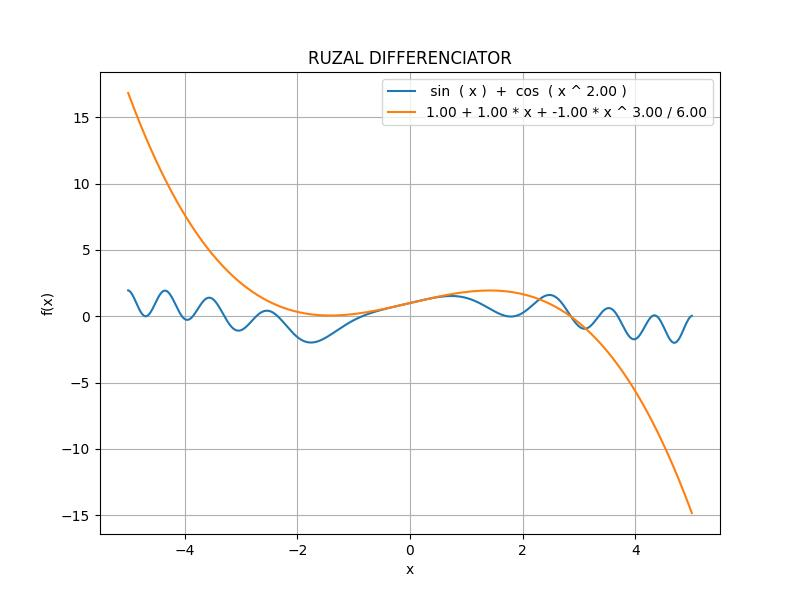
\includegraphics[scale = 0.700000]{teylor.jpeg}
\end{flushleft}
\end{figure}
\end{document}